\documentclass{ieeeaccess}

\usepackage{cite}
\usepackage{amsmath,amssymb,amsfonts}
\usepackage{graphicx}
\usepackage{booktabs}
\usepackage{multirow}
\usepackage{array}
\usepackage{url}
\usepackage{float}
\usepackage{textcomp}

\newdimen\xfigwd
\xfigwd=\columnwidth

\def\BibTeX{{\rm B\kern-.05em{\sc i\kern-.025em b}\kern-.08em
    T\kern-.1667em\lower.7ex\hbox{E}\kern-.125emX}}

\begin{document}

\history{Date of publication xxxx 00, 0000, date of current version xxxx 00, 0000.}
\doi{10.1109/ACCESS.2026.DOI}

\title{Depth-Guided and Tree-Focused Learning for Tree Classification under Complex Backgrounds}

\author{\uppercase{Takahiro Matsumura}\authorrefmark{1}}

\address[1]{Affiliation to be confirmed. The source PDF metadata lists Takahiro Matsumura as the author.}

\tfootnote{This manuscript reorganizes the content of the source paper \texttt{vit-mil-conference-template-a4.pdf} into the IEEE Access \LaTeX{} template. Author affiliations and correspondence details should be verified before submission.}

\markboth
{T. Matsumura: Depth-Guided and Tree-Focused Learning for Tree Classification under Complex Backgrounds}
{T. Matsumura: Depth-Guided and Tree-Focused Learning for Tree Classification under Complex Backgrounds}

\corresp{Corresponding author: Takahiro Matsumura (contact details to be confirmed).}

\begin{abstract}
Tree classification in urban and orchard environments plays an important role in landscape management, agricultural support, and environmental monitoring. However, tree images captured from mid-range distances often include extensive background regions, leading models to overfit contextual information rather than intrinsic features such as trunks and branches. In this study, we propose a trunk-focused learning framework that integrates the Vision Transformer (ViT) with attention-based multiple instance learning (ABMIL). Furthermore, we introduce Depth-guided Attention and Depth-guided Augmentation, which incorporate depth maps estimated by the MiDaS model into both data augmentation and attention computation stages to guide the model's focus toward foreground structures such as trunks and branches. Comparative experiments were conducted on 16 configurations using the FruitsPark dataset collected at Fuefuki Fruits Park, Yamanashi Prefecture, Japan, and the UrbanStreetTree dataset containing urban street tree images from China. The proposed depth-guided methods significantly outperformed conventional CNN and ViT models, achieving accuracies of up to 97.9\% on the UrbanStreetTree dataset and 95.2\% on the FruitsPark dataset. Visualization of attention maps further confirmed stable focus on trunk and branch regions facilitated by depth information, suggesting that depth signals serve as an effective auxiliary cue for suppressing background dependency.
\end{abstract}

\begin{keywords}
Attention-based multiple instance learning, background suppression, depth-guided attention, depth-guided augmentation, tree classification, urban forestry, Vision Transformer.
\end{keywords}

\titlepgskip=-15pt
\maketitle

\section{Introduction}
\label{sec:introduction}

Automatic classification of urban and orchard trees plays an important role in landscape management, agricultural support, and environmental monitoring within smart-city frameworks \cite{b4,b5,b6,b7}. Previous studies have mainly focused on classifying leaves, flowers, fruits, or close-up images of tree trunks \cite{b5,b6,b7,b9,b10}. However, in practical applications, close-range images of target trees are not always available, and it is often necessary to use mid-range images captured from a certain distance, as illustrated in Fig.~\ref{fig:distance_examples}.

\begin{figure}[t]
\centering
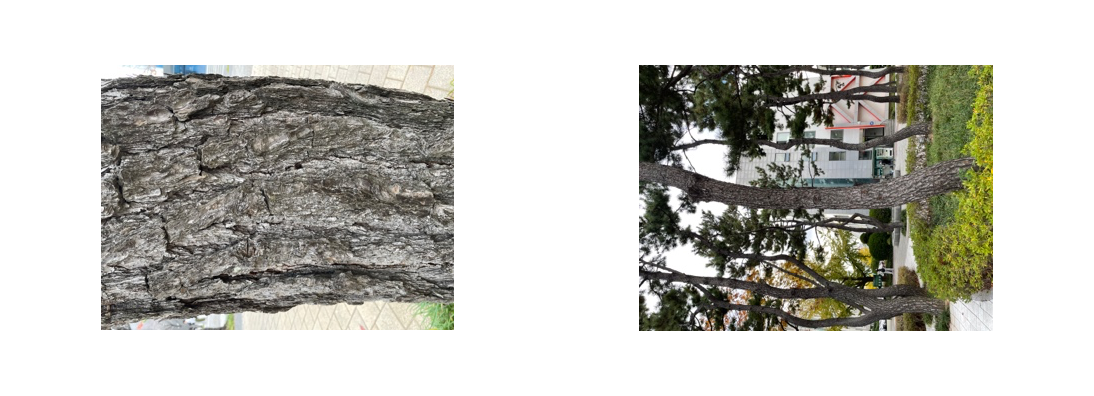
\includegraphics[width=0.9\columnwidth]{figures/fig01_samples.png}
\caption{Sample images of tree trunks captured at different distances.}
\label{fig:distance_examples}
\end{figure}

In mid-range images, trees occupy only a small portion of the frame, and large background regions are inevitably included. As a result, learning models tend to depend heavily on background features. High classification accuracy can sometimes be achieved using background information alone, which creates the risk that a model overfits contextual patterns rather than intrinsic features such as trunks and leaves. This effect becomes particularly severe when models are trained on small datasets collected from limited viewpoints or locations, where background diversity is low. Conversely, datasets captured under diverse environmental conditions are expected to mitigate such background bias.

Moreover, species classification from mid-range images often requires manual annotation of trunk regions, which remains a labor-intensive and costly process. The distance between the camera and the tree, as well as the image resolution, also significantly affects bark texture. For example, two trunks that appear to have the same width in an image may represent completely different textures, such as a thin trunk captured at close range and a thick trunk photographed from afar, as illustrated in Figs.~\ref{fig:distance_problem} and \ref{fig:texture_problem}. This issue, referred to here as the texture degradation and distance inconsistency problem, is a major challenge in mid-range tree recognition.

\begin{figure}[t]
\centering
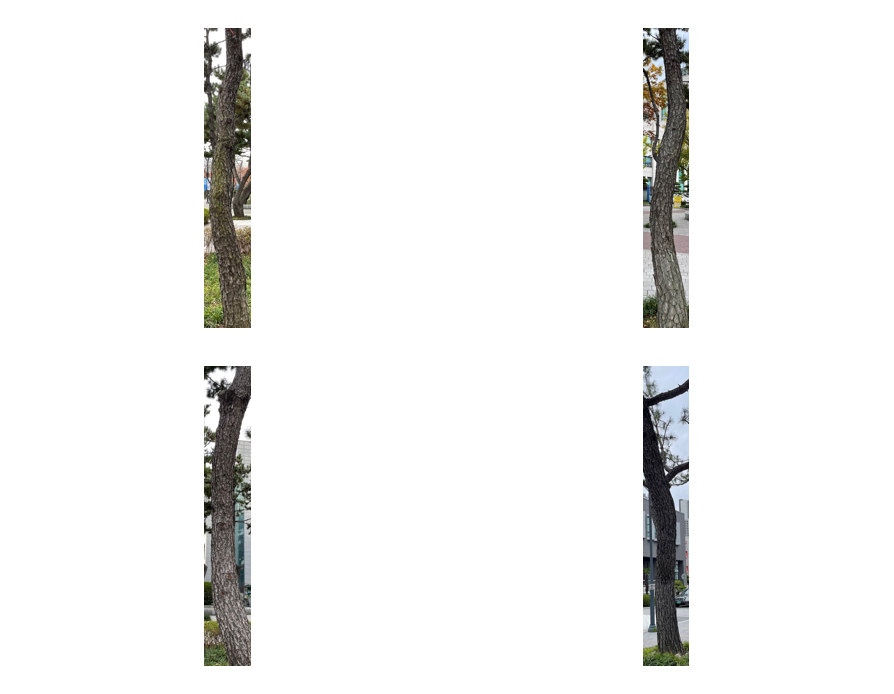
\includegraphics[width=\columnwidth]{figures/fig02_distance_inconsistency.png}
\caption{Texture degradation and distance inconsistency problem in mid-range tree images. Each example shows a tree trunk with a different diameter and capture distance.}
\label{fig:distance_problem}
\end{figure}

\begin{figure}[t]
\centering
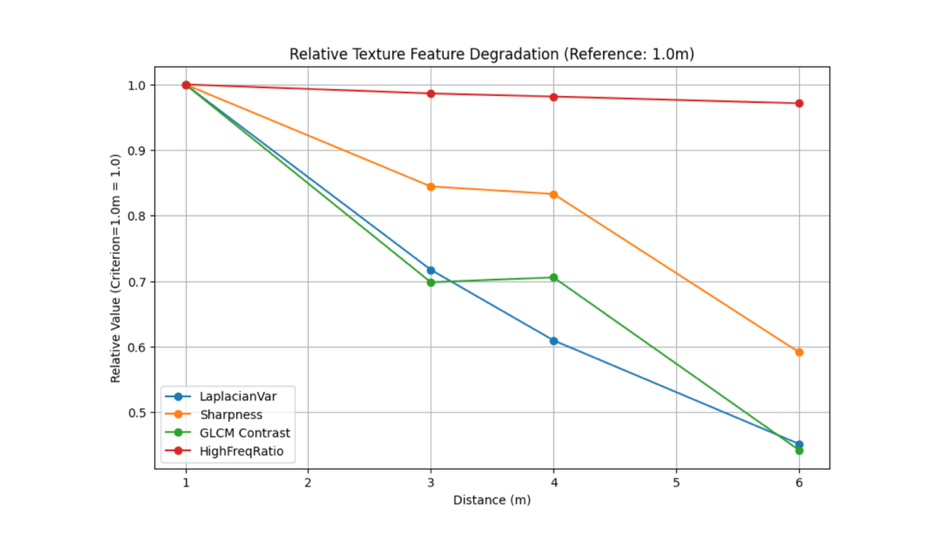
\includegraphics[width=\columnwidth]{figures/fig03_texture_degradation.png}
\caption{Relative texture feature degradation caused by image scale and shooting distance.}
\label{fig:texture_problem}
\end{figure}

To address these issues, this study proposes a classification framework that integrates the Vision Transformer (ViT) \cite{b1} with attention-based multiple instance learning (ABMIL) \cite{b2}. The goal is to emphasize intrinsic tree features such as trunks and branches while suppressing background interference in mid-range images. In addition, the framework incorporates depth estimation based on MiDaS \cite{b3} and background-suppression mechanisms such as top-$k$ selection and Laplacian-based filtering to reduce background bias and achieve more robust tree classification across diverse environments.

\section{Related Work}
\label{sec:relatedwork}

\subsection{Significance of Tree Species Classification and Conventional Approaches}
Tree species classification in urban environments is a fundamental technology for landscape management and conservation planning \cite{b4}. In recent years, automatic identification using smartphone applications has become increasingly common. Representative systems include LeafSnap \cite{b5}, Pl@ntNet \cite{b6}, and Folia \cite{b7}. These tools are widely used by citizens and in educational settings, providing an accessible platform for understanding urban biodiversity even for non-specialists. However, most of these applications rely primarily on close-up images, and research focusing on mid- or long-range observations remains limited. Furthermore, many existing methods require manual annotation for supervised classification, which raises labeling costs in practical use.

\subsection{Commonly Used Features and Limitations of Existing Datasets}
Typical morphological features used for tree classification include leaves, bark, leaf shapes, flowers, and fruits. Among these, leaves are the most commonly used because they are easy to observe. Large-scale datasets such as Pl@ntLeaves \cite{b8} and LeafSnap \cite{b5} have contributed to the prevalence of leaf-based classification studies. However, leaves, flowers, and fruits are highly seasonal and cannot be used during leaf-off or non-flowering periods. In contrast, bark can be observed year-round and is therefore a promising feature independent of seasonal variation. Public datasets such as BarkNet 1.0 \cite{b9} and Bark-101 \cite{b10} have facilitated progress in bark-based classification research. Nevertheless, most of these datasets consist of close-up images captured under conditions with minimal background interference. When relying solely on texture features, differences between bark textures of various species can be subtle, and classification becomes even more challenging as trees age. Moreover, when trunks are photographed from mid- to long-range distances, variations in shooting distance and image resolution significantly affect texture representation, leading to severe accuracy degradation.

\subsection{Urban Tree Datasets and Future Directions}
Most existing tree datasets have been independently collected by individual researchers, resulting in limited interoperability and comparability across studies \cite{b4}. In contrast, the UrbanStreetTree dataset \cite{b11}, developed for urban street trees in China, covers multiple tree organs, including trunks, leaves, whole trees, branches, flowers, and fruits, and contains 41,467 images. A distinctive feature of that dataset is its detailed annotation of branch structures, which enables species identification even under challenging conditions such as winter leaf-off periods or painted trunks.

\subsection{Positioning of This Study}
To address the challenges described above, this study combines ViT \cite{b1} with ABMIL \cite{b2} to reduce background dependency and encourage the model to focus on trunk regions. MIL-based patch division allows the model to retain high-resolution local information while avoiding information loss due to aggressive resizing, thereby facilitating attention to fine-grained features even in long-distance images. By further leveraging the self-attention mechanism of the Transformer architecture, the proposed framework can simultaneously capture both local bark texture and global tree structure, leading to more robust and context-aware tree classification.

\section{Method}
\label{sec:method}

\subsection{Overview of the Method}
This study focuses on the effect of incorporating depth information at different stages and compares four model configurations, including those without depth usage. Depth maps are estimated and optionally employed either as auxiliary input signals or as attention guidance during learning. The common framework is shown in Fig.~\ref{fig:framework}. In all cases, depth information is used only during training, while inference is performed solely with RGB images. Although depth maps can theoretically be employed as additional inputs, they are often unavailable or unreliable in real-world settings. Therefore, this study adopts a training-only strategy that leverages depth as structural supervision, improving generalizability and practical usability by eliminating dependence on depth estimation during inference.

\begin{figure*}[t]
\centering
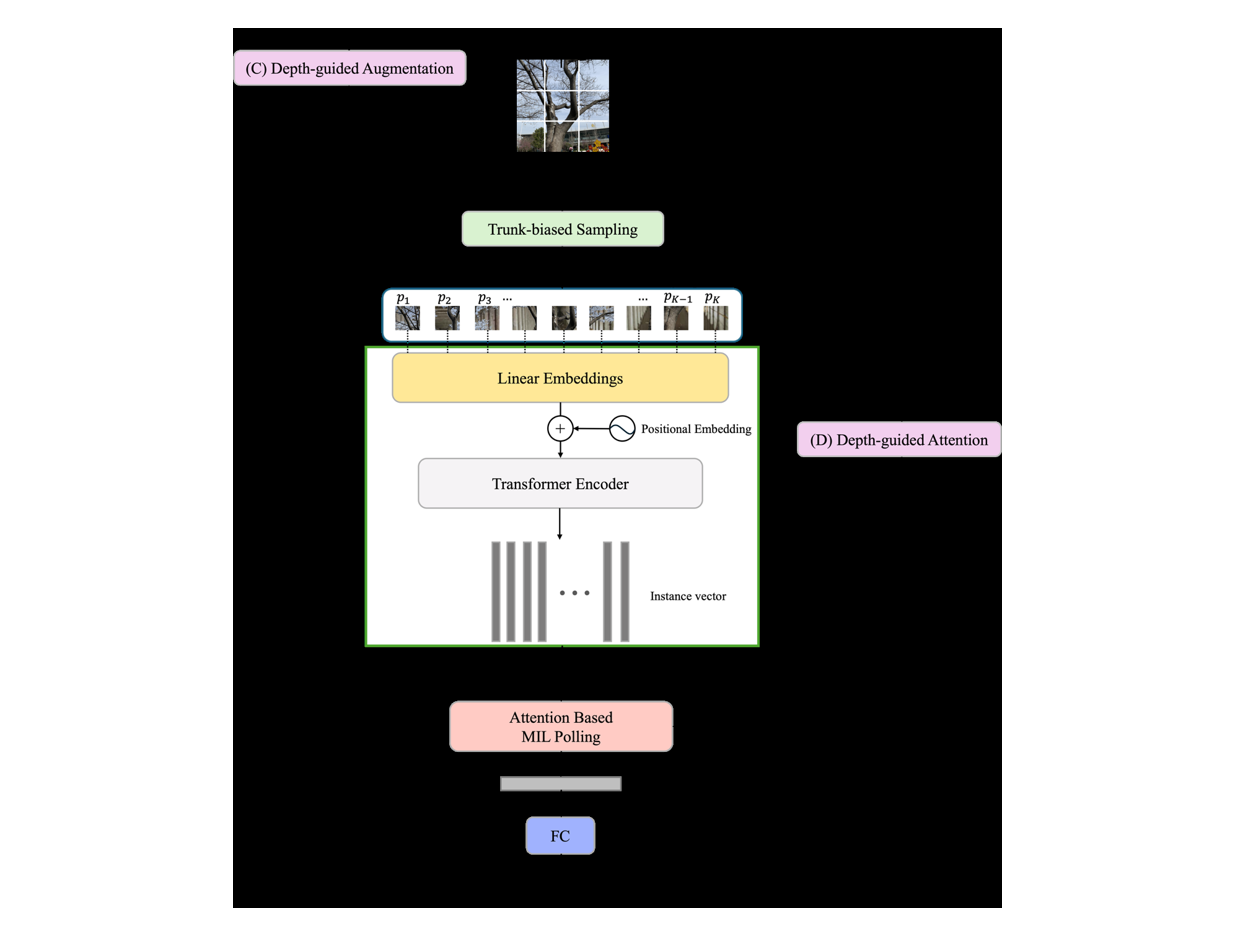
\includegraphics[width=\textwidth]{figures/fig04_framework.png}
\caption{Overview of the proposed classification framework based on ViT and MIL. The configuration without depth usage corresponds to ViT + MIL. Two depth-guided extensions are also considered: Depth-guided Augmentation and Depth-guided Attention. Both approaches use depth information only during training.}
\label{fig:framework}
\end{figure*}

The four configurations are summarized as follows.
\begin{enumerate}
\item \textbf{Baseline:} the input image is directly fed to ResNet18 \cite{b12}, ViT \cite{b1}, or DINO-pretrained ViT \cite{b13}, and classification is performed with either global average pooling (GAP) or ABMIL. No depth information is used.
\item \textbf{ViT + MIL:} ViT is combined with MIL to process images at the patch level and automatically extract informative regions such as trunks, branches, and leaves.
\item \textbf{Depth-guided Augmentation:} depth maps are used to preserve near-field regions while varying far-field regions at the input stage, so the model implicitly learns to focus on the foreground.
\item \textbf{Depth-guided Attention:} depth maps are incorporated into the attention computation to suppress distant background regions and emphasize near-field structures.
\end{enumerate}

\subsection{Classification Using ViT + ABMIL}
Given an input image $x$, the image is divided into $N$ patches of size $P \times P$, and each patch $p_i$ is mapped into a feature space through the ViT embedding function $\phi(\cdot)$:
\begin{equation}
z_i = \phi(p_i) \in \mathbb{R}^{d}, \qquad i=1,\ldots,N.
\label{eq:patch_embedding}
\end{equation}
The resulting feature set $Z = [z_1,\ldots,z_N]$ is processed by ABMIL using the attention score
\begin{equation}
e_i = w^{\top} \tanh(W z_i + b),
\label{eq:mil_score}
\end{equation}
followed by temperature-scaled normalization,
\begin{equation}
a_i = \frac{\exp(e_i / \tau)}{\sum_{j=1}^{N} \exp(e_j / \tau)},
\label{eq:mil_attention}
\end{equation}
where $W$, $w$, and $b$ are learnable parameters and $\tau$ controls the sharpness of the attention distribution. In this study, the standard softmax can be replaced by entmax or top-$k$ normalization to obtain sparse attention and emphasize salient local regions.

The bag-level representation is given by
\begin{equation}
s = \sum_{i=1}^{N} a_i z_i,
\label{eq:bag_representation}
\end{equation}
and class probabilities are computed as
\begin{equation}
p(y=c\mid x) = \mathrm{softmax}(W_c s + b_c).
\label{eq:classification}
\end{equation}
The classification loss is the cross-entropy
\begin{equation}
L_{\mathrm{cls}} = -\sum_{c} y_c \log p(y=c\mid x).
\label{eq:cross_entropy}
\end{equation}
This formulation allows ABMIL to selectively emphasize important regions within ViT-extracted patch features, enabling the model to focus on structural information such as trunks and branches while reducing reliance on background cues.

To prioritize highly textured regions such as tree trunks and bark, a trunk-biased sampling strategy is introduced in the ABMIL instance-generation process. For a candidate patch set $\mathcal{C}$ produced by a sliding window, a texture score $S(q)$ is computed for each patch $q \in \mathcal{C}$ using one of the following indicators:
\begin{align}
S_{\mathrm{lapvar}}(q) &= \mathrm{Var}[\mathrm{Laplacian}(q)],
\label{eq:lapvar}\\
S_{\mathrm{sobel}}(q) &= \mathbb{E}[\lVert \nabla q \rVert_2],
\label{eq:sobel}\\
S_{\mathrm{hpf}}(q) &= \mathbb{E}[(\mathrm{HPF}(q))^2].
\label{eq:hpf}
\end{align}
The default metric is Laplacian variance. Patches are sorted in descending order of $S(q)$, and the top $\lfloor K\beta \rfloor$ patches are deterministically selected, where $\beta$ denotes the trunk-bias ratio. The remaining $K-\lfloor K\beta \rfloor$ patches are sampled uniformly from the rest to preserve bag diversity. During training, this trunk-biased sliding sampler is alternated with random sampling in mixed mode to balance structural emphasis and diversity.

The final loss combines the bag-level classification loss with regularization terms controlling sparsity and smoothness of the attention distribution:
\begin{equation}
L = L_{\mathrm{cls}} + \lambda_{\mathrm{ent}} H(A) + \lambda_{1} \lVert A \rVert_{1},
\label{eq:regularized_loss}
\end{equation}
where
\begin{equation}
H(A) = -\sum_i A_i \log(A_i + \varepsilon).
\label{eq:entropy}
\end{equation}
The entropy term suppresses excessive concentration, while the $L_1$ term promotes sparsity and encourages the model to focus on a limited number of informative patches.

\subsection{Depth-Guided Augmentation}
During training, depth-guided augmentation is probabilistically applied using relative depth maps estimated by MiDaS \cite{b3}. Foreground regions corresponding to trunks and branches are preserved, while background regions are replaced or degraded using external natural images. Boundary transitions are smoothed through morphological operations and feathering, and standard photometric augmentations such as blur, color transformation, and JPEG compression are applied to expand variation in background and illumination conditions. This approach aims to prevent overfitting to background diversity inherent in mid-range tree images and to guide model attention consistently toward intrinsic structures. The augmentation is applied only to training data; validation and test data remain unchanged.

\subsection{Depth-Guided Attention}
In the Depth-guided Attention model, depth information is incorporated directly into attention computation. Depth guidance is active only during training, whereas inference uses standard MIL-based attention without depth input. Let $D_i$ denote the mean normalized depth value of patch $i$ in the range $[0,1]$. The depth weighting function is defined as
\begin{equation}
g(D_i) =
\begin{cases}
1, & D_i \le t,\\
\exp\{-\gamma(D_i-t)\}, & D_i > t,
\end{cases}
\label{eq:depth_weight}
\end{equation}
where $t$ is the threshold and $\gamma$ controls the decay rate. This prior assigns higher weights to near-field trunk regions and exponentially suppresses distant background contributions.

At the score level, depth is integrated by late fusion,
\begin{equation}
e_i \leftarrow e_i + \eta \log(g_i + \varepsilon),
\label{eq:late_fusion}
\end{equation}
where $\eta$ is the fusion strength. After attention normalization, a geometric-mean fusion variant is also considered:
\begin{equation}
\tilde{A}_i = \frac{A_i^{1-\lambda} g_i^{\lambda}}{\sum_j A_j^{1-\lambda} g_j^{\lambda}},
\label{eq:geometric_fusion}
\end{equation}
where $\lambda$ controls the contribution of depth. This formulation preserves the learned attention structure while enhancing emphasis on near-field trunk regions.

\section{Datasets}
\label{sec:datasets}

This study uses two datasets: a dataset independently collected in Japan (FruitsPark) and a publicly available urban tree dataset (UrbanStreetTree).

\subsection{FruitsPark Dataset}
The FruitsPark dataset was independently collected at a public fruit park in Japan between June 2024 and May 2025 as part of a field survey conducted in a designated experimental area. It consists of images from ten tree classes. Images were captured using an iPhone 15 Pro and a Pixel 7 Pro and unified to a resolution of $1080 \times 1920$ pixels. The dataset covers all four seasons and includes diverse backgrounds such as soil, other trees, playground equipment, and signboards within the park. To prevent data leakage between training and validation, samples were divided by individual trees and collection periods. Sample images are shown in Fig.~\ref{fig:fruitspark_samples}.

\begin{figure*}[t]
\centering
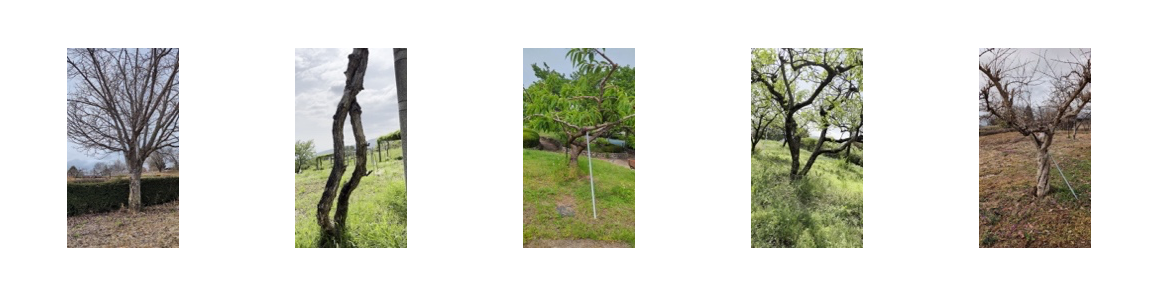
\includegraphics[width=\textwidth]{figures/fig05_fruitspark.png}
\caption{Sample images from the FruitsPark dataset.}
\label{fig:fruitspark_samples}
\end{figure*}

\subsection{UrbanStreetTree Dataset}
The UrbanStreetTree dataset (Branch subset) consists of urban street tree images collected across ten cities in China \cite{b11}. Images were captured using multiple devices at a resolution of $3008 \times 3970$ pixels. Because the dataset includes mid-range images with people, vehicles, and buildings in the background, it is well suited for evaluating classification performance in complex urban environments. Sample images are shown in Fig.~\ref{fig:urbanstreettree_samples}.

\begin{figure*}[t]
\centering
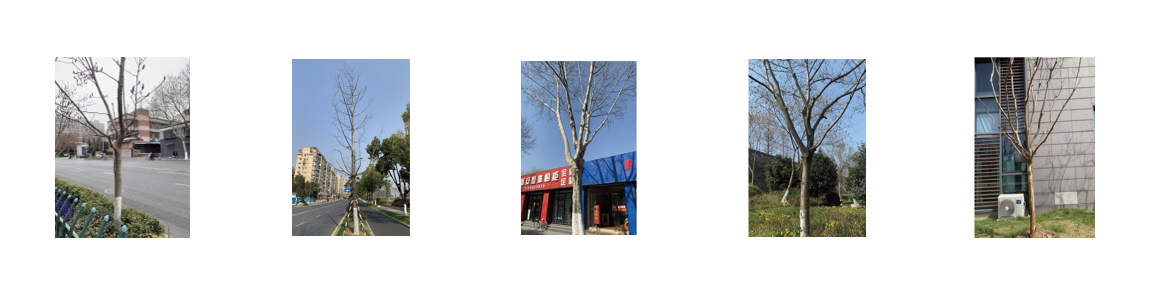
\includegraphics[width=\textwidth]{figures/fig06_urbanstreettree.png}
\caption{Sample images from the UrbanStreetTree dataset \cite{b11}.}
\label{fig:urbanstreettree_samples}
\end{figure*}

\subsection{Data Augmentation and Dataset Comparison}
During training, two augmentation policies are considered.
\begin{enumerate}
\item \textbf{Standard photometric augmentation:} random brightness and contrast adjustment ($\pm 0.2$), hue-saturation-value transformation, motion blur (3--5 pixels), resizing to $224 \times 224$, and ImageNet normalization.
\item \textbf{Depth-based background replacement:} foreground tree regions are preserved, while background regions are replaced with external natural scenes according to the estimated depth map. Morphological operations and feathering are used to maintain smooth boundaries.
\end{enumerate}
Representative images generated by the depth-guided augmentation process are shown in Fig.~\ref{fig:depth_aug_samples}.

\begin{figure*}[t]
\centering
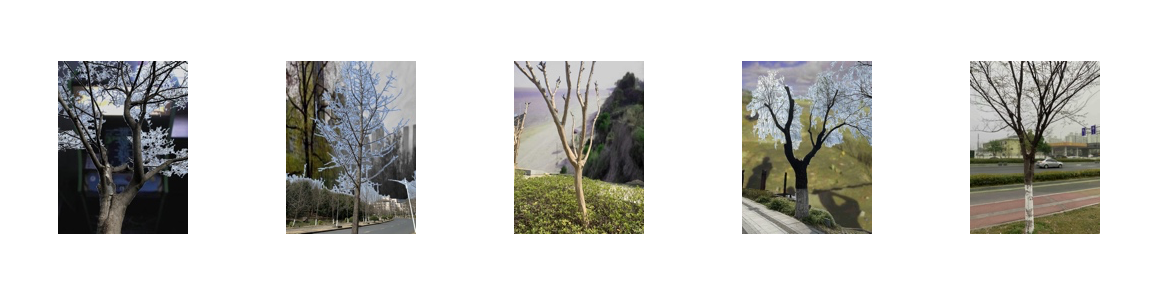
\includegraphics[width=\textwidth]{figures/fig07_depth_aug.png}
\caption{Sample images generated by depth-guided augmentation.}
\label{fig:depth_aug_samples}
\end{figure*}

Table~\ref{tab:depth_aug_config} summarizes the detailed augmentation settings. Tables~\ref{tab:data_split} and \ref{tab:dataset_compare} summarize the dataset split and dataset characteristics used throughout the experiments.

\begin{table*}[t]
\centering
\caption{Configuration of depth-guided background replacement augmentation.}
\label{tab:depth_aug_config}
\resizebox{\textwidth}{!}{%
\begin{tabular}{p{5.2cm}p{8.8cm}c}
\toprule
Processing step & Description / setting & Probability \\
\midrule
Depth estimation and foreground extraction & Depth estimated using MiDaS (DPT-Hybrid); the foreground tree region is extracted and only the largest connected component is retained. & 100\% \\
Background replacement & Background is replaced with natural scenes from the Places365 dataset, with depth matching enabled. & 80\% \\
Mask processing & Erosion: 5 px; dilation: 3 px; feathering: 13 px. & 100\% \\
Blur effect & Gaussian blur with strength 3--10. & 90\% \\
Color transformation & Brightness, contrast, and saturation scaled by 0.65--1.35; hue shifted by $\pm 0.10$. & 55\% \\
JPEG compression & JPEG compression with quality 16--50. & 70\% \\
\bottomrule
\end{tabular}}
\end{table*}

\begin{table*}[t]
\centering
\caption{Data splits before and after augmentation.}
\label{tab:data_split}
\resizebox{0.75\textwidth}{!}{%
\begin{tabular}{lccc}
\toprule
Dataset & Train & Validation & Test \\
\midrule
FruitsPark (original) & 580 & 210 & 0 \\
FruitsPark (augmented) & 2,273 & 210 & 0 \\
UrbanStreetTree (original) & 1,193 & 149 & 143 \\
UrbanStreetTree (augmented) & 4,674 & 149 & 143 \\
\bottomrule
\end{tabular}}
\end{table*}

\begin{table*}[t]
\centering
\caption{Comparison of the datasets used in this study.}
\label{tab:dataset_compare}
\resizebox{\textwidth}{!}{%
\begin{tabular}{p{3.2cm}p{5.2cm}p{6.0cm}}
\toprule
Item & FruitsPark & UrbanStreetTree \\
\midrule
Number of classes & 10 & 13 \\
Number of images & 790 & 1,485 \\
Number of images (augmented) & 2,483 & 4,966 \\
Data split & Training and validation (no test set) & Training, validation, and test \\
Image resolution & $1080 \times 1920$ px & $3008 \times 3970$ px \\
Aspect ratio & 0.562 & 0.760 \\
Class distribution & Uniform (246--251 images per class, $\pm 3$) & Diverse (minimum 299, maximum 581 per class) \\
Shooting conditions & Inside a park, 3--5 m distance; multiple seasons and times; backgrounds include playgrounds and signboards & Urban streets, 0.1--3 m distance; multiple seasons and cities; backgrounds include people, vehicles, and buildings \\
Capture devices & iPhone 15 Pro and Pixel 7 Pro & Multiple mobile devices \\
\bottomrule
\end{tabular}}
\end{table*}

\section{Results}
\label{sec:results}

\subsection{Models and Comparative Methods}
The effectiveness of depth guidance was evaluated with Transformer-based models as the primary focus. The base models were ResNet18 \cite{b12}, ViT \cite{b1}, and Swin Transformer \cite{b14}. For ViT, the study additionally used a DINO-pretrained model initialized with weights learned on ImageNet-1K \cite{b13}. In total, 16 configurations were compared: ResNet18 with GAP or MIL, ViT and DINO-ViT with GAP or MIL, depth-guided variants, and Swin Transformer with MIL.

\subsection{Evaluation Metrics}
Classification performance was evaluated with accuracy and micro-averaged $F_1$ score on the test dataset. If no separate test set was available, the validation dataset was used instead. Attention maps were also visualized to qualitatively analyze how depth guidance altered attention distributions.

Accuracy is defined as
\begin{equation}
\mathrm{Accuracy} = \frac{1}{N} \sum_{i=1}^{N} \mathbf{1}(\hat{y}_i = y_i),
\label{eq:accuracy}
\end{equation}
where $N$ is the total number of samples, $y_i$ is the ground-truth label, and $\hat{y}_i$ is the predicted label. The micro-$F_1$ score is computed as
\begin{equation}
\mathrm{Micro\mbox{-}F_1} = \frac{2\,TP}{2\,TP + FP + FN}.
\label{eq:microf1}
\end{equation}

\subsection{Overall Results}
Table~\ref{tab:main_results} summarizes the classification results on FruitsPark and UrbanStreetTree. Overall, Transformer-based models significantly outperformed ResNet-based models, and the depth-guided variants achieved the best results on both datasets.

\begin{table*}[t]
\centering
\caption{Classification results on UrbanStreetTree and FruitsPark.}
\label{tab:main_results}
\resizebox{\textwidth}{!}{%
\begin{tabular}{clcccc}
\toprule
\multirow{2}{*}{Category} & \multirow{2}{*}{Method} & \multicolumn{2}{c}{UrbanStreetTree} & \multicolumn{2}{c}{FruitsPark} \\
\cmidrule(lr){3-4}\cmidrule(lr){5-6}
 &  & Accuracy (\%) & Micro-$F_1$ (\%) & Accuracy (\%) & Micro-$F_1$ (\%) \\
\midrule
\multirow{4}{*}{Baseline} 
& ResNet18 + GAP & 87.25 & 82.52 & 90.00 & 90.00 \\
& ResNet18 + MIL & 64.00 & 64.34 & 61.90 & 61.90 \\
& ViT + GAP & 79.20 & 74.80 & 89.00 & 88.30 \\
& ViT (DINO) + GAP & 66.43 & 62.00 & 78.09 & 78.00 \\
\midrule
\multirow{3}{*}{ViT + MIL}
& ViT + MIL & 90.91 & 88.66 & 86.19 & 86.05 \\
& ViT (DINO) + MIL & 80.00 & 80.00 & 74.82 & 70.00 \\
& Swin + MIL & 74.50 & 73.27 & 87.62 & 86.98 \\
\midrule
\multirow{3}{*}{Depth Augmentation}
& ViT + MIL & 94.41 & 93.84 & 95.24 & 95.16 \\
& ViT (DINO) + MIL & 97.90 & 97.76 & 91.90 & 91.89 \\
& Swin + MIL & 90.21 & 87.49 & 85.24 & 80.16 \\
\midrule
\multirow{6}{*}{Depth-guided Attention}
& ViT + MIL & 91.61 & 90.23 & 90.48 & 90.37 \\
& ViT (DINO) + MIL & 93.71 & 92.64 & 91.90 & 91.72 \\
& ViT + MIL + Late Fusion & 90.91 & 89.24 & 85.24 & 84.84 \\
& ViT (DINO) + MIL + Late Fusion & 91.61 & 89.20 & 90.48 & 90.14 \\
& ViT + MIL + Piecewise Depth & 93.01 & 90.91 & 88.57 & 88.52 \\
& ViT (DINO) + MIL + Piecewise Depth & 93.71 & 92.82 & 88.57 & 88.41 \\
\bottomrule
\end{tabular}}
\end{table*}

\subsection{Baseline Comparison}
ResNet18 with simple GAP achieved high accuracy---87.25\% on UrbanStreetTree and 90.00\% on FruitsPark---but showed signs of overfitting to training data. When the MIL structure was introduced, performance dropped substantially: ResNet18 + MIL achieved only 64.00\% on UrbanStreetTree and 61.90\% on FruitsPark. For ViT, the GAP configuration yielded slightly lower accuracy than ResNet18. However, when MIL was combined with ViT, accuracy improved to 90.91\% on UrbanStreetTree and 86.19\% on FruitsPark, indicating that multi-region aggregation contributed positively to performance.

\subsection{Effect of DINO Pretraining}
When the self-supervised DINO-pretrained ViT was used, accuracy decreased significantly in the GAP configuration. Compared with the standard ViT baseline, DINO-ViT dropped by 12.77 points on UrbanStreetTree and 10.91 points on FruitsPark. A similar trend appeared in the MIL configuration. However, in settings that incorporated depth information, DINO-based models consistently improved performance on several tasks. This suggests that DINO's global representation becomes more useful when constrained by depth guidance.

\subsection{Effect of Depth Guidance}
Depth-based augmentation produced the strongest improvements overall. ViT (DINO) + MIL + Depth Augmentation achieved 97.90\% on UrbanStreetTree, while ViT + MIL + Depth Augmentation achieved 95.24\% on FruitsPark. Regardless of DINO pretraining, depth-guided augmentation proved effective across both datasets. All depth-guided models outperformed their corresponding baselines on UrbanStreetTree. On FruitsPark, more than half of the depth-guided models improved upon their reference baselines, although the degree of improvement varied with environmental conditions.

\subsection{Effects of Late Fusion and Piecewise Depth}
Late Fusion generally yielded lower accuracies than the corresponding depth-guided attention models without post-processing, suggesting that direct logarithmic addition of depth weights does not stabilize the attention distribution. Piecewise Depth provided small improvements on UrbanStreetTree but reduced stability on FruitsPark. Overall, the experimental results suggest that Late Fusion tends to degrade performance, whereas Piecewise Depth has dataset-dependent effects.

\subsection{Qualitative Evaluation}
Attention maps were used to examine whether the proposed framework actually focused on the target tree rather than the background. In the baseline ResNet + GAP model, strong attention frequently fell on buildings, roads, unrelated trees, and poles. ViT + MIL still exhibited broadly distributed attention over background elements. In contrast, the depth-guided models concentrated attention on foreground structures such as trunks, branches, and leaves while reducing dispersion to the background. This trend was consistent across both datasets.

\begin{figure*}[t]
\centering
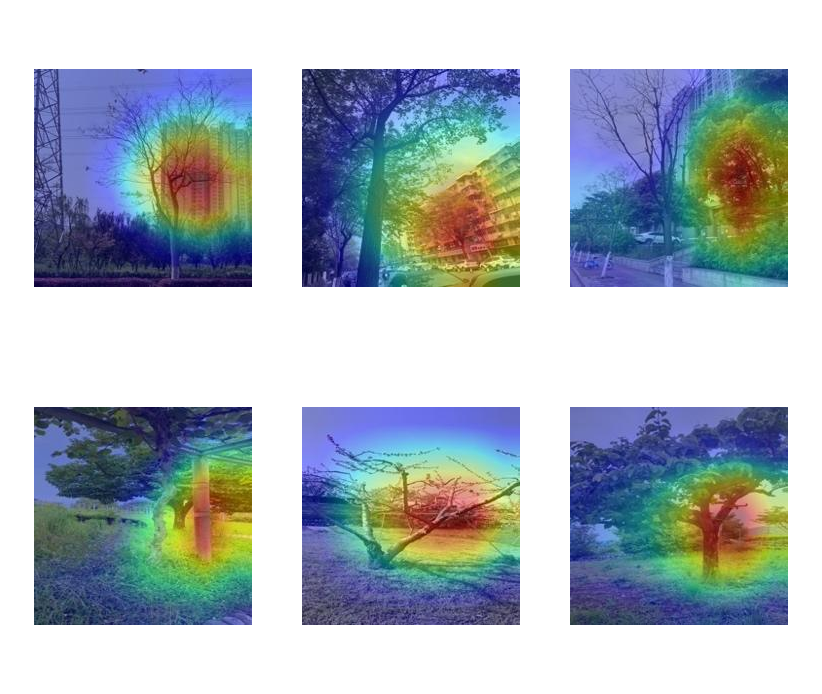
\includegraphics[width=\textwidth]{figures/fig08_resnet_gap_attention.png}
\caption{Samples of attention maps for ResNet + GAP (Method 1).}
\label{fig:attn_resnet}
\end{figure*}

\begin{figure*}[t]
\centering
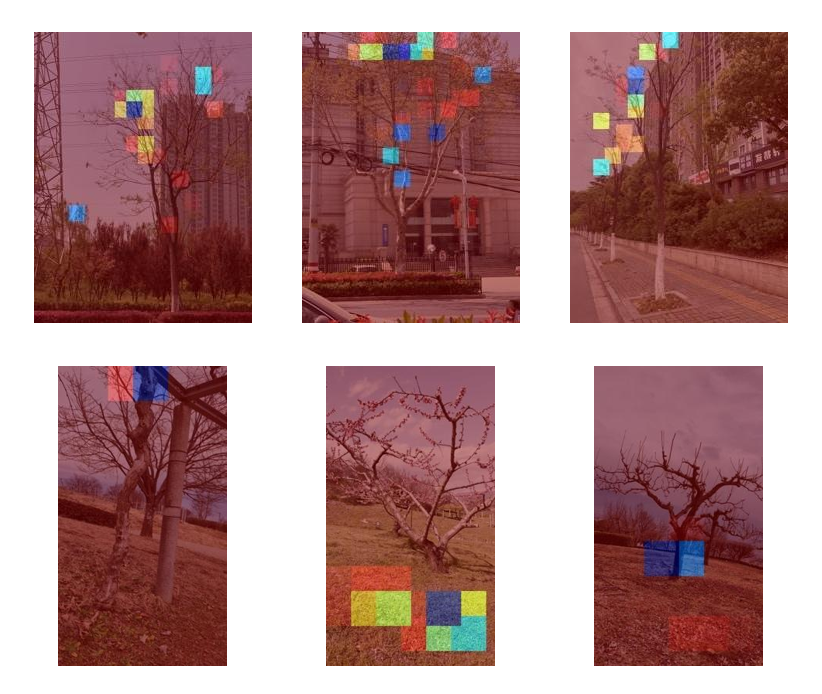
\includegraphics[width=\textwidth]{figures/fig09_vit_mil_attention.png}
\caption{Samples of attention maps for ViT + MIL (Method 5).}
\label{fig:attn_vitmil}
\end{figure*}

\begin{figure*}[t]
\centering
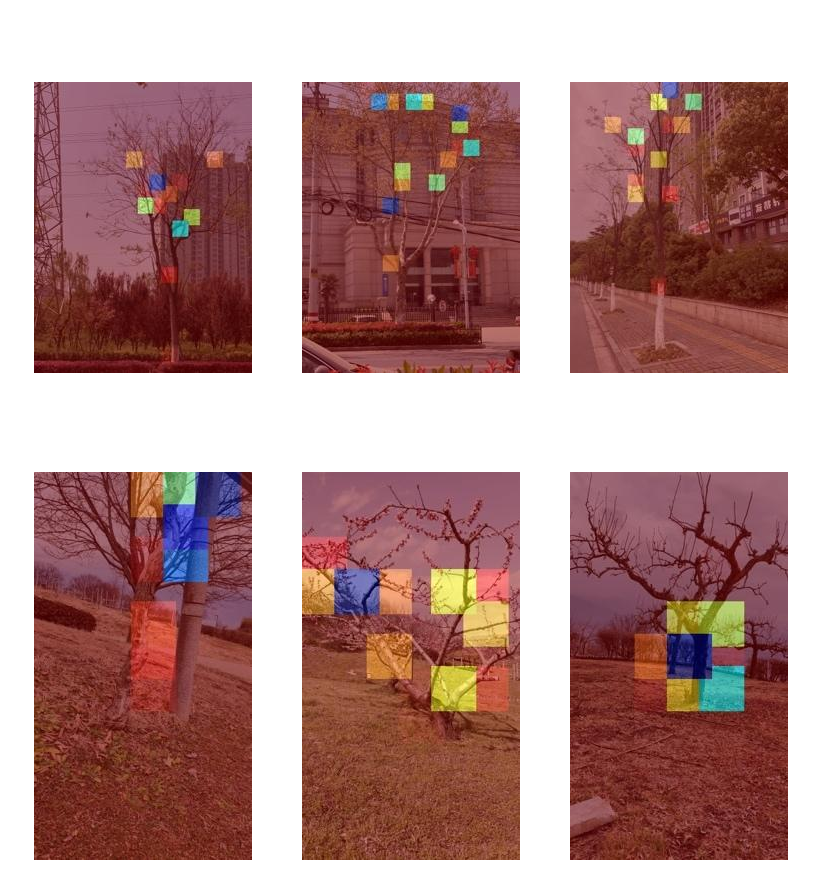
\includegraphics[width=\textwidth]{figures/fig10_vit_mil_depth_aug_attention.png}
\caption{Samples of attention maps for ViT + MIL + Depth Augmentation (Method 8).}
\label{fig:attn_depthaug}
\end{figure*}

\begin{figure*}[t]
\centering
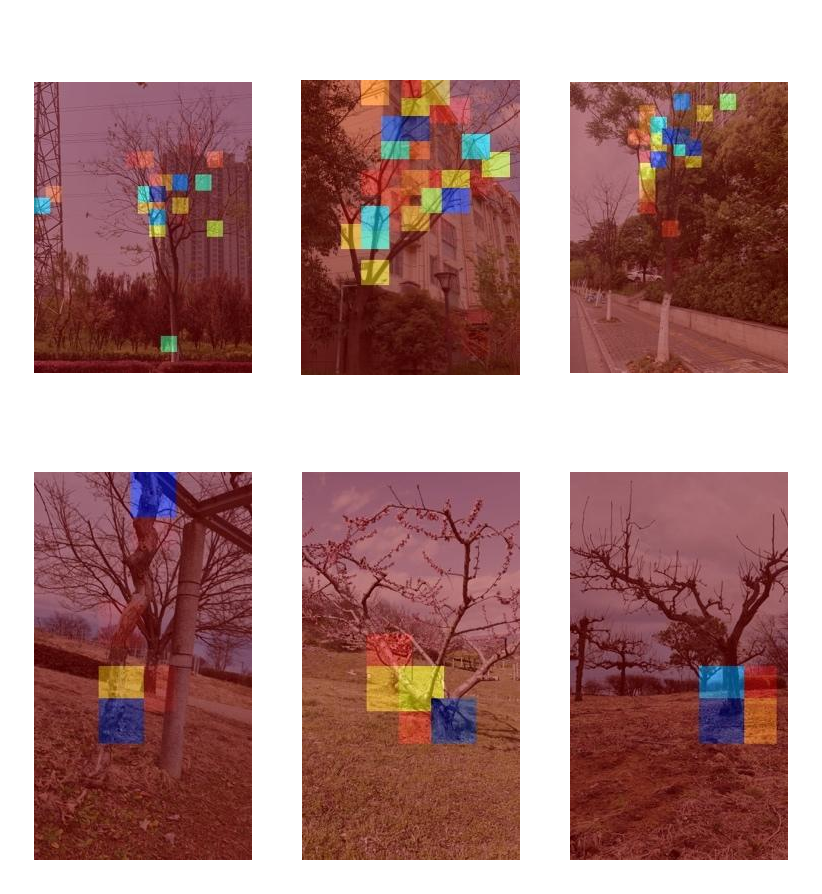
\includegraphics[width=\textwidth]{figures/fig11_dino_depth_aug_attention.png}
\caption{Samples of attention maps for ViT (DINO) + MIL + Depth Augmentation (Method 9).}
\label{fig:attn_dino_depthaug}
\end{figure*}

\begin{figure*}[t]
\centering
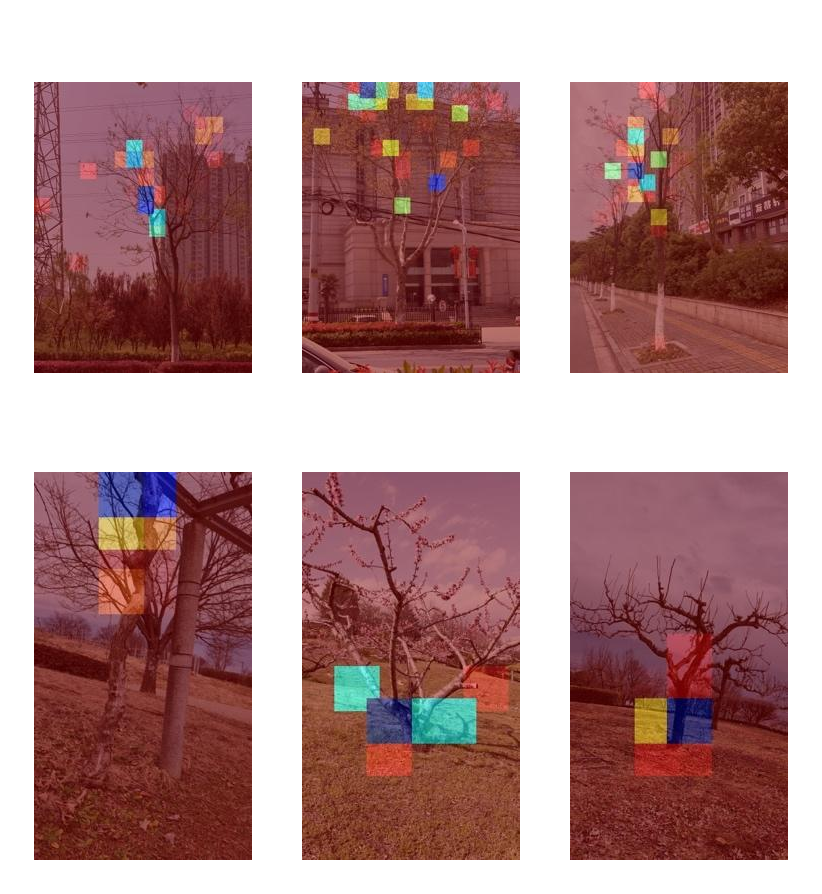
\includegraphics[width=\textwidth]{figures/fig12_depth_attention.png}
\caption{Samples of attention maps for ViT + MIL + Depth-guided Attention (Method 11).}
\label{fig:attn_depthattention}
\end{figure*}

\begin{figure*}[t]
\centering
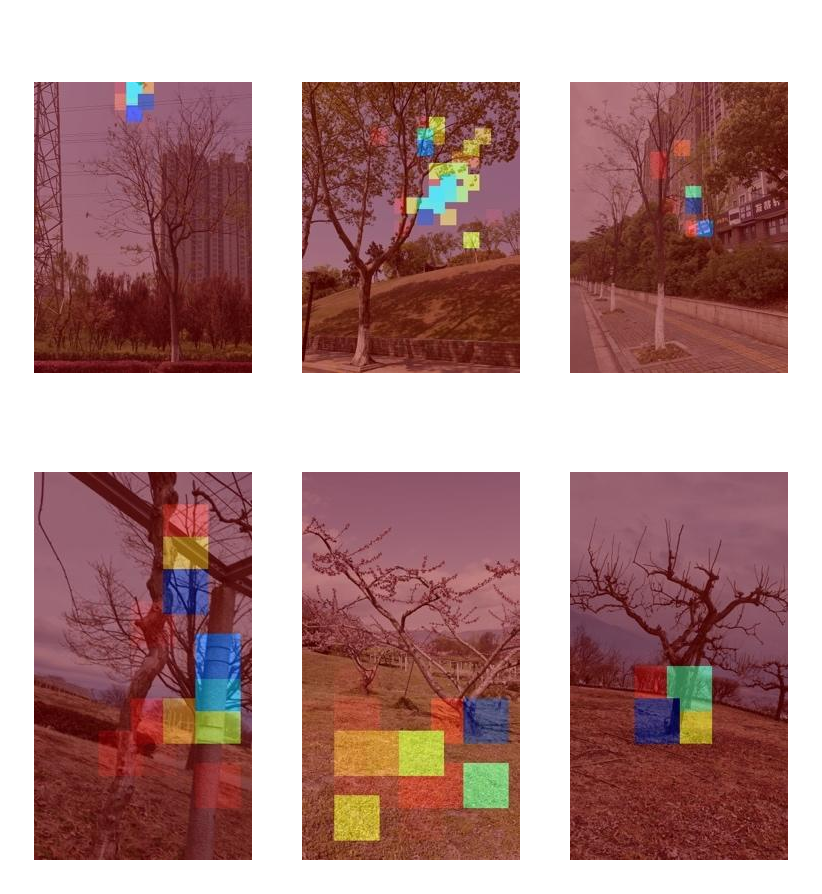
\includegraphics[width=\textwidth]{figures/fig13_latefusion_attention.png}
\caption{Samples of attention maps for ViT + MIL + Depth-guided Attention + Late Fusion (Method 13).}
\label{fig:attn_latefusion}
\end{figure*}

\begin{figure*}[t]
\centering
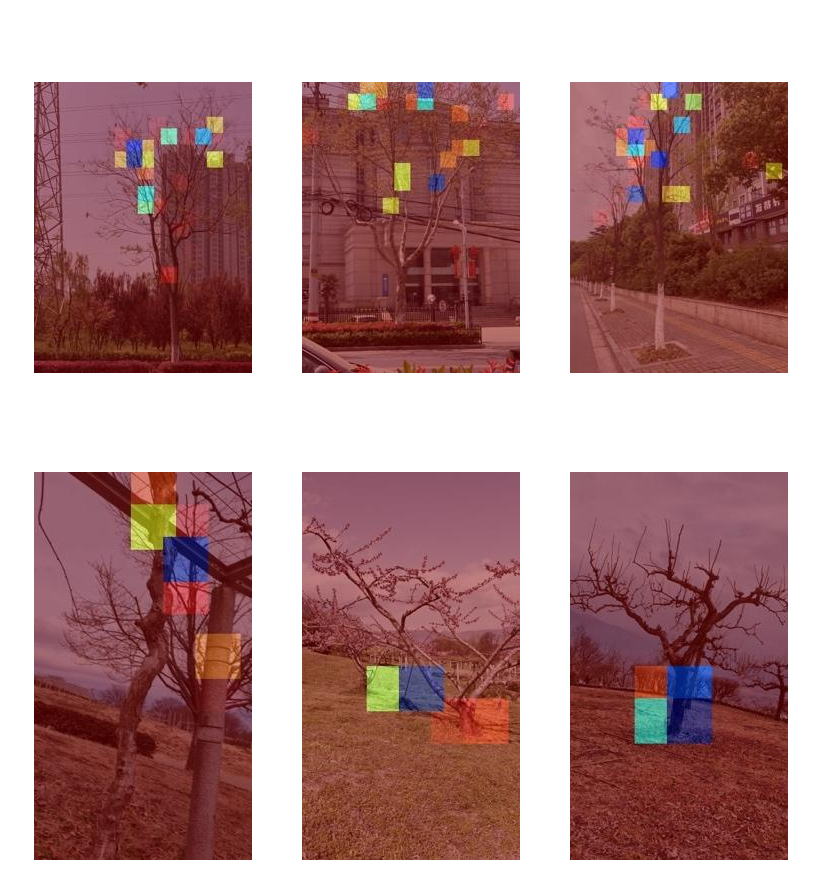
\includegraphics[width=\textwidth]{figures/fig14_piecewise_attention.png}
\caption{Samples of attention maps for ViT + MIL + Depth-guided Attention + Piecewise Depth (Method 15).}
\label{fig:attn_piecewise}
\end{figure*}

\section{Discussion}
\label{sec:discussion}

\subsection{Factors Contributing to Performance Improvement by Depth Guidance}
Methods incorporating depth information---namely Depth-guided Attention and Depth-guided Augmentation---consistently achieved higher classification accuracy than ResNet18 and standard ViT. These results indicate that depth guidance suppresses the influence of background regions and directs attention toward foreground structures such as trunks, branches, and leaves. In particular, Depth-guided Augmentation enables simulation of diverse environmental conditions through background replacement, promoting robust feature learning that is less dependent on contextual background information. The qualitative visualization results support this interpretation because the depth-guided models exhibit stronger focus on the foreground.

Although Depth-guided Attention showed smaller improvement margins than Depth-guided Augmentation, it maintained stable foreground focus during inference. This suggests that integrating depth directly into the model architecture, rather than relying solely on data augmentation, offers a generalizable and deployable strategy for real-world applications.

\subsection{Influence of DINO Pretraining}
Self-supervised pretraining with DINO enables the model to learn global structural representations from large-scale natural images without label supervision \cite{b13}. However, DINO tends to prioritize global scene consistency over local object details. When applied to tree images where foreground and background are tightly entangled, attention often spreads across background areas. This explains the degraded performance observed in configurations without depth guidance. In contrast, when depth guidance was combined with DINO, performance improved in most settings. DINO's global representation captures holistic scene structure, while depth information acts as a local suppression signal that reweights features toward the foreground.

\subsection{Stability of Late Fusion and Piecewise Depth}
Introducing Late Fusion consistently degraded accuracy. The logarithmic combination of depth weights alters the relative strength of attention scores, causing the attention distribution either to overexpand or to become locally biased. Attention map visualization also revealed attention drifting toward the ground and background, suggesting that simple additive fusion disrupts scale consistency between depth and feature representations.

Piecewise Depth produced limited improvement on UrbanStreetTree but decreased accuracy on FruitsPark. This discrepancy likely stems from differences in object distance and background composition between datasets, implying that a single discretization threshold cannot be applied universally. To make the piecewise approach more effective, dynamic segmentation or learnable optimization based on depth distribution appears necessary.

\subsection{Dataset Characteristics and Generalization}
While all depth-guided methods improved accuracy on UrbanStreetTree, several configurations led to degraded performance on FruitsPark. This can be attributed to the diverse illumination conditions, seasonal variations, and nearby ground and neighboring trees in FruitsPark, all of which introduce strong visual noise. Such environmental complexity can cause the depth estimation model to misclassify foreground and background regions, thereby reducing the reliability of depth-based attention guidance. Consequently, the effectiveness of depth guidance strongly depends on the quality of depth estimation and the stability of environmental imaging conditions.

\section{Conclusion}
\label{sec:conclusion}

This study verified the effectiveness of integrating depth information into Transformer-based models for tree image classification, with particular attention to foreground enhancement and background suppression. Experimental results demonstrated that depth-guided approaches consistently outperformed ResNet and standard ViT baselines. In particular, the Depth-guided Attention structure exhibited stable and consistent performance as an architectural extension. These findings suggest that depth information is highly compatible with the self-attention mechanism of Transformers and serves as an effective auxiliary signal for extracting key structures under varying background conditions.

Conversely, simple additive fusion methods such as Late Fusion and Piecewise Depth tended to destabilize attention by disrupting the scale consistency of depth features. Effective integration of depth information therefore requires not a static arithmetic combination, but a context-aware and dynamically optimized design that adapts to the feature distribution.

\subsection{Future Work}
Future research should incorporate confidence-aware depth weighting and dynamically adaptive depth-integration modules within the Transformer architecture. In addition, the MiDaS model used in this study produces pseudo-depth maps inferred from RGB images rather than absolute distance measurements. Further experiments using physically measured depth data, such as LiDAR or stereo cameras, would provide more rigorous validation of depth-guided learning. Developing domain-specific depth estimation models optimized for particular environments, such as orchards, and extending the approach to other outdoor natural objects would also help evaluate the generalization potential of depth-assisted visual understanding.

\begin{thebibliography}{00}

\bibitem{b1} A. Dosovitskiy \emph{et al.}, ``An Image Is Worth 16$\times$16 Words: Transformers for Image Recognition at Scale,'' in \emph{Proc. Int. Conf. Learn. Representations (ICLR)}, 2021.

\bibitem{b2} J. Peters, S. Wild, and L. Schmidt, ``Attention-Based Multiple Instance Learning for Visual Recognition,'' in \emph{Proc. Int. Conf. Mach. Learn. (ICML)}, 2019, pp. 7745--7755.

\bibitem{b3} R. Ranftl, K. Lasinger, D. Hafner, K. Schindler, and V. Koltun, ``MiDaS: Towards High-Quality Monocular Depth Estimation,'' in \emph{Proc. IEEE Conf. Comput. Vis. Pattern Recognit. Workshops (CVPRW)}, 2020, pp. 131--144.

\bibitem{b4} B. Robert, M. David, and A. Martin, ``Challenges in Tree Species Identification from Mid-Range Images: Dataset Interoperability and Standardization,'' \emph{Ecol. Inform.}, vol. 60, Art. no. 101284, 2020.

\bibitem{b5} N. Kumar, P. N. Belhumeur, A. Biswas, D. W. Jacobs, W. J. Kress, I. C. Lopez, and J. V. Soares, ``Leafsnap: A Computer Vision System for Automatic Plant Species Identification,'' in \emph{Proc. Eur. Conf. Comput. Vis. (ECCV)}, 2012, pp. 502--516.

\bibitem{b6} H. Go\"eau, P. Bonnet, and A. Joly, ``Plant Identification in an Open World (Pl@ntNet),'' in \emph{Proc. Eur. Conf. Comput. Vis. Workshops (ECCVW)}, 2013, pp. 21--33.

\bibitem{b7} R. Cerutti, L. Tougne, A. Vacavant, and D. Coquin, ``Folia: An Application for Plant Identification Using Leaf Image Analysis,'' in \emph{Proc. Int. Conf. Image Anal. Recognit. (ICIAR)}, 2013, pp. 527--534.

\bibitem{b8} H. Go\"eau, P. Bonnet, A. Joly, V. Baki\'c, J. Barbe, S. Selmi, I. Yahiaoui, and A. Barth\'el\'emy, ``Pl@ntLeaves: A Leaf Image Database,'' in \emph{Proc. Int. Conf. Multimedia Retr.}, 2012.

\bibitem{b9} M. Carpentier, P. Gigu\`ere, and J. Gaudreault, ``BarkNet 1.0: A Dataset for Bark Classification,'' \emph{arXiv preprint arXiv:1806.03474}, 2018.

\bibitem{b10} M. Ratajczak, M. Kozio\l{}, and A. Koz\l{}owski, ``Bark-101: A Dataset for Bark Species Classification Using Deep Convolutional Neural Networks,'' in \emph{Proc. Int. Conf. Image Process. (ICIP)}, 2019, pp. 103--107.

\bibitem{b11} T. Kim, Y. Zhang, and Q. Wang, ``UrbanStreetTree: A Large-Scale Dataset for Urban Tree Species Classification and Segmentation,'' \emph{Remote Sens.}, vol. 14, no. 4, Art. no. 932, 2022.

\bibitem{b12} K. He, X. Zhang, S. Ren, and J. Sun, ``Deep Residual Learning for Image Recognition,'' in \emph{Proc. IEEE Conf. Comput. Vis. Pattern Recognit. (CVPR)}, 2016, pp. 770--778.

\bibitem{b13} M. Caron, H. Touvron, I. Misra, H. J\'egou, J. Mairal, P. Bojanowski, and A. Joulin, ``Emerging Properties in Self-Supervised Vision Transformers,'' in \emph{Proc. IEEE Int. Conf. Comput. Vis. (ICCV)}, 2021, pp. 9650--9660.

\bibitem{b14} Z. Liu \emph{et al.}, ``Swin Transformer: Hierarchical Vision Transformer Using Shifted Windows,'' in \emph{Proc. IEEE Int. Conf. Comput. Vis. (ICCV)}, 2021, pp. 10012--10022.

\end{thebibliography}

\EOD

\end{document}
